\chapter{Peaks}
\label{Peaks}
\graphicspath{{Figures/Peaks/}}

The results presented in this chapter have been published in \citet{Dall:2009}. All of the theoretical work in this paper except as noted in this chapter was my own work.

\section{The metastable Helium Peaks experiment}
\label{Peaks:ExperimentalSetup}

\begin{figure}[htbp]
    \centering
        \includegraphics[height=3in]{ExperimentalResults}
    \caption{Experimental results. The difference between (a) and (b) is that the outcoupling Rabi frequency has been increased by an order of magnitude in (b).}
    \label{Peaks:ExperimentalResults}
\end{figure}

\begin{figure}[htbp]
    \centering
        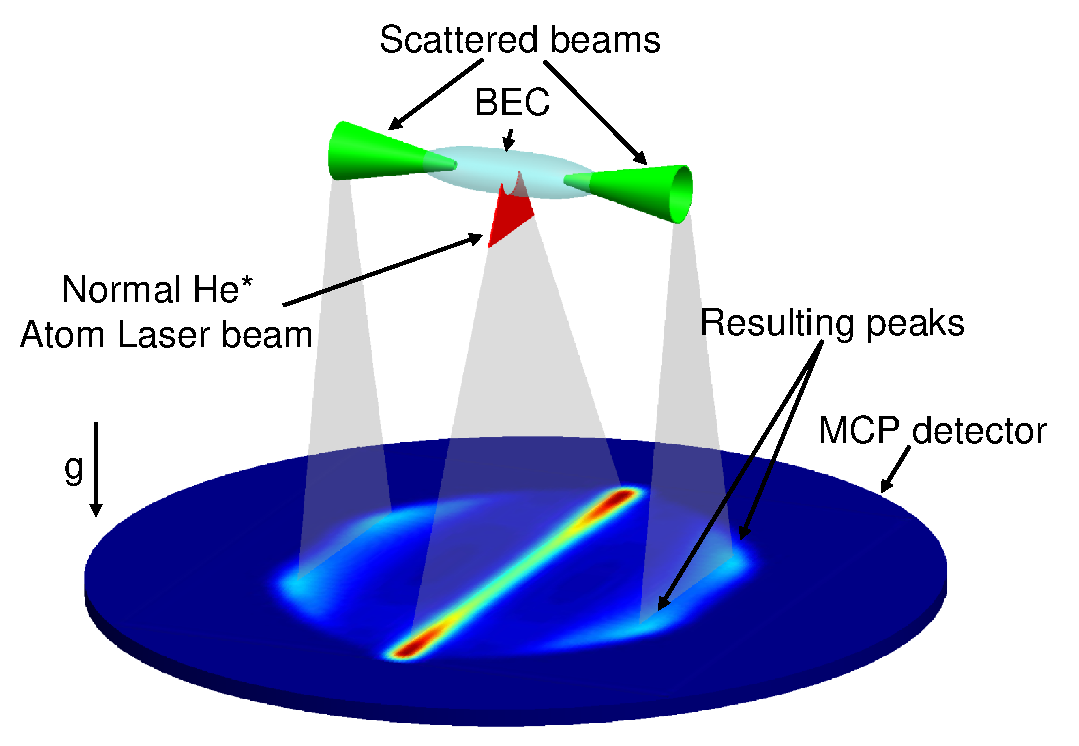
\includegraphics[height=3in]{Schematic}
    \caption{Schematic of the experimental setup}
    \label{Peaks:Schematic}
\end{figure}


\begin{table}
    \centering
    \begin{tabular}{cc}
    \toprule
    Parameter & Value\\
    \midrule
    r2c1 & r2c2\\
    r3c1 & r3c2\\
    r4c1 & r4c2\\
    r5c1 & r5c2\\
    r6c1 & r6c2\\
    \bottomrule
    \end{tabular}
    \caption{Experimental Parameters for the metastable Helium BEC under consideration.}
    \label{Peaks:ExperimentalParameters}
\end{table}




% FIXME: Somewhere in the experimental results we need to state that the momentum of the excitation in the weak trapping dimension is larger than the momentum width in the weak trapping dimension suggesting that something significant is happening along that axis. 

\section{Quasiparticle excitation spectrum (All hail the Bog-meister)}

%While the argument in the previous section gives a qualitative explanation for the four-wave mixing process observed in He*, it is not entirely satisfying. In this section an approximate analytic expression for the excited modes of the He* system will be obtained and investigated using Bogoliubov stuff.

The experimental results presented in the previous section are caused by a dynamical instability that causes the formation of excitations within the condensate.  In this section, the response of the condensate to small perturbations will be studied to discover the nature and origin of this instability. This study will take the form of a derivation of the dispersion relation for the fundamental excitations of the condensate within the framework of the Bogoliubov method \citep{Bogoliubov:1947,FetterWalecka}.

The Bogoliubov procedure \citep{Bogoliubov:1947} is to approximate and then diagonalise the Hamiltonian to obtain the energy spectrum of the fundamental excitations of the condensate, known as \emph{quasiparticles}.  Applying this procedure directly to the Hamiltonian itself leads to a Hamiltonian that doesn't conserve number. There are various ways of approaching this problem \citep{FetterWalecka}, but the one used here will be to take the chemical potentials $\mu_i$ as given quantities, from which the number can be obtained consistently.

In taking the chemical potentials as prescribed, it is the grand-canonical Hamiltonian $\displaystyle\protect{\hat{K} \equiv \hat{H} - \sum_i \mu_i \hat{N}_i}$ that we will approximate and diagonalise.  The condensate density in this experiment isn't uniform, however if the excitations under consideration have wavelengths much smaller than the Thomas-Fermi radius then the quasiparticle excitation spectrum is well-described within the local density approximation (LDA) \citep{Stamper-Kurn:1999,Zambelli:2000} in which the condensate is assumed to be homogeneous.  It is expected that the LDA will hold for this system as from the experimental results it can be seen that the momentum of the excitations in the weak trapping dimension is larger than the momentum width of the condensate in that dimension\footnote{FIXME: Once the experimental results are in, this bit will need changing}, hence the wavelength of the excitation in that dimension will be less than the Thomas-Fermi radius.


We take as our system the two interacting states $m_F=1, 0$ neglecting the antitrapped state $m_F=-1$ as it is expected to have negligible density. The grand-canonical Hamiltonian for this system is,
\begin{align}
    \hat{K} &\equiv \hat{H} - \sum_i \mu_i \hat{N}_i\\
            &= \sum_i \int d\mathbf{x}\, \hat{\Psi}_i^\dagger \left(\frac{-\hbar^2 \nabla^2}{2 M} - \mu_i\right)\hat{\Psi}_i + \frac{1}{2} \sum_{i j} U_{i j}\int d\mathbf{x}\, \hat{\Psi}_i^\dagger \hat{\Psi}_j^\dagger \hat{\Psi}_j \hat{\Psi}_i,
\end{align}
where $\hat{H}$ is the usual Hamiltonian operator, $\displaystyle\hat{N}_i= \int d\mathbf{x}\, \hat{\Psi}_i^\dagger \hat{\Psi}_i$ is the number operator, $\mu_i$ is the chemical potential for the $m_F=i$ state, $U_{ij} = 4\pi \hbar^2 a_{ij}/M$ is the nonlinear interaction strength, $a_{ij}$ is the s-wave scattering length between internal states $i$ and $j$. In this Hamiltonian the Rabi coupling between the $m_F$ levels has been neglected as it will be a perturbation to the system driving longer timescale dynamics. Instead the aim here is to investigate the original cause for the production of the observed excitations.

The Bogoliubov approximation separates the highly-occupied zero-momentum groundstate mode from the fluctuations about that mode by defining deviation operators $\delta\hat{\Psi}_i = \hat{\Psi}_i - \mean{\hat{\Psi}_i}$ and then treating $\delta\hat{\Psi}_i$ as a small quantity. These fluctuation operators obey the boson commutation relations $\comm{\delta\hat{\Psi}_i(\mathbf{x}), \delta \hat{\Psi}_j^\dagger(\mathbf{x}')} = \delta_{i j} \delta(\mathbf{x}-\mathbf{x}')$. To simplify notation the expectation value of the atomic field will be written as $\mean{\hat{\Psi}_i} = \Psi_i$ where $\Psi_i$ can be taken to be real due to the phase symmetry of the grand canonical Hamiltonian $\hat{K}$.

Making this replacement and keeping terms up to second order in the fluctuation operators gives
\begin{align}
    \begin{split}
        \hat{K} =& -\sum_i \mu_i N_i^{(0)} + \frac{1}{2}\sum_{i j}U_{i j}\int d\mathbf{x} \abs{\Psi_i}^2\abs{\Psi_j}^2 + \sum_i \int d\mathbf{x}\, \delta\hat{\Psi}_i^\dagger \left( \frac{-\hbar^2 \nabla^2}{2M} - \mu_i\right)\delta\hat{\Psi}_i\\
        &+ \sum_{i j} U_{i j} \int d\mathbf{x}\, \Big[\Psi_j^2\delta\hat{\Psi}_i^\dagger \delta\hat{\Psi}_i + \Psi_i\Psi_j\Big(\delta\hat{\Psi}_i^\dagger \delta\hat{\Psi}_j + \frac{1}{2} \delta\hat{\Psi}_i^\dagger \delta\hat{\Psi}_j^\dagger + \frac{1}{2}\delta\hat{\Psi}_i \delta\hat{\Psi}_j \Big)\Big],
    \end{split}
\end{align}
where $N_i^{(0)}$ is the number of atoms in the ground state. There are no terms linear in $\delta\hat{\Psi}_i^{(\dagger)}$ in this expression as they are all of the form
\begin{align}
    \sum_i \int d\mathbf{x}\,  \bigg( \frac{-\hbar^2 \nabla^2}{2M}\Psi_i - \mu_i\Psi_i + \frac{1}{2} \sum_j U_{i j} \abs{\Psi_j}^2\Psi_i\bigg) \delta \hat{\Psi}_i^\dagger, \label{Peaks:ConstantAndQuadraticK}
\end{align}
where the term in parentheses is zero by assumption that the mean field $\Psi_i$ represents the ground state of the $m_F=i$ state with energy $\mu_i$. The constant terms in \eqref{Peaks:ConstantAndQuadraticK} only contribute a physically meaningless overall energy offset. The remaining quadratic terms in the grand canonical Hamiltonian are
\begin{align}
    \begin{split}
        \hat{K}' =& \sum_i \int d\mathbf{x}\, \delta\hat{\Psi}_i^\dagger \left( \frac{-\hbar^2 \nabla^2}{2M} - \mu_i\right)\delta\hat{\Psi}_i\\
        &+ \sum_{i j} U_{i j} \int d\mathbf{x}\, \Big[\Psi_j^2\delta\hat{\Psi}_i^\dagger \delta\hat{\Psi}_i + \Psi_i\Psi_j\Big(\delta\hat{\Psi}_i^\dagger \delta\hat{\Psi}_j +\frac{1}{2} \delta\hat{\Psi}_i^\dagger \delta\hat{\Psi}_j^\dagger +  \frac{1}{2}\delta\hat{\Psi}_i \delta\hat{\Psi}_j \Big)\Big].
    \end{split}
    \label{Peaks:QuadraticK}
\end{align}

As this system is translation-invariant, the grand-canonical Hamiltonian takes its simplest form in a Fourier basis. Performing the Fourier transform of \eqref{Peaks:QuadraticK} gives
\begin{align}
    \begin{split}
        \hat{K}' =& \sum_i \int d\mathbf{k}\, \bigg(\frac{\hbar^2 \mathbf{k}^2}{2M} - \mu_i + \sum_j U_{ij} \Psi_j^2\bigg) \delta\hat{\Psi}_i^\dagger(\mathbf{k}) \delta\hat{\Psi}_i(\mathbf{k}) \\
        &+ \sum_{i j} U_{i j}\Psi_i \Psi_j\int d\mathbf{k}\, \Big( \delta\hat{\Psi}_i^\dagger(\mathbf{k}) \delta\hat{\Psi}_j(\mathbf{k}) + \frac{1}{2}\delta\hat{\Psi}_i^\dagger(\mathbf{k}) \delta\hat{\Psi}_j^\dagger (-\mathbf{k}) + \frac{1}{2} \delta\hat{\Psi}_i(\mathbf{k}) \delta\hat{\Psi}_j(-\mathbf{k})\Big) .
    \end{split}
    \label{Peaks:QuadraticKKSpace}
\end{align}

In order to extract the quasiparticle excitation spectrum we wish to transform this quadratic Hamiltonian into the diagonal form
\begin{align}
    \hat{K}' &= \sum_n \int d\mathbf{q}\, E_n(\mathbf{q}) \hat{\Phi}_n^\dagger(\mathbf{q}) \hat{\Phi}_n(\mathbf{q}) \label{Peaks:DesiredQuadraticForm}
\end{align}
for some continuous variable $\mathbf{q}$, discrete index $n$ and field operators $\hat{\Phi}_n(\mathbf{q})$ satisfying the boson commutation relations. For single-component systems this is usually achieved by making the Bogoliubov transform
\begin{align}
    \hat{\Psi}(\mathbf{k}) &= u(\mathbf{k}) \hat{\Phi}(\mathbf{k}) - v(\mathbf{k}) \hat{\Phi}^\dagger(-\mathbf{k}), \label{Peaks:BogoliubovTransformation}
\end{align}
for some real functions $u(\mathbf{k})$, $v(\mathbf{k})$. It is not clear how this will proceed for multi-component systems particularly as it is expected that an individual quasiparticle excitation will include excitations in both internal states.

Instead we proceed by following the procedure of \citep{Leonhardt:2003} and recasting the problem as an eigenvalue problem by considering the Heisenberg evolution equation for an arbitrary operator $\hat{Q}$,
\begin{align}
    \frac{d \hat{Q}}{dt} &= \frac{i}{\hbar}\comm{\hat{K}', \hat{Q}}. \label{Peaks:HeisenbergEvolution}
\end{align}
The operators $\hat{\Phi}_n(\mathbf{q})$ defined in \eqref{Peaks:DesiredQuadraticForm} evolve according to \eqref{Peaks:HeisenbergEvolution} as
\begin{align}
    \frac{d \hat{\Phi}_n(\mathbf{q})}{dt} &= \frac{i}{\hbar}\comm{\hat{K}', \hat{\Phi}_n(\mathbf{q})} = - \frac{i}{\hbar} E_n(\mathbf{q}) \hat{\Phi}_n(\mathbf{q}).
\end{align}
Expanding the $\hat{\Phi}_n(\mathbf{q})$ in terms of the complete basis $\big\{\delta\hat{\Psi}_i(\mathbf{k}), \delta\hat{\Psi}_i^\dagger(\mathbf{k}): i \in \{0, 1\}, \mathbf{k} \in \mathbb{R}^3\big\}$ gives an eigenvalue problem with eigenvalue $-\frac{i}{\hbar}E_n(\mathbf{q})$.  At first glance this appears to be an infinite dimensional eigenvalue problem due to the infinite range of $\mathbf{k}$. As can be seen from \eqref{Peaks:QuadraticKKSpace} however, the fields $\delta\hat{\Psi}_i^{(\dagger)}(\mathbf{k})$ only couple to  $\delta\hat{\Psi}_j^{(\dagger)}(-\mathbf{k})$ reducing the problem to a finite-dimensional eigenvalue problem for each $\mathbf{k}$. Further, evaluating the commutator in \eqref{Peaks:HeisenbergEvolution} for the deviation operator $\delta\hat{\Psi}_i(\mathbf{k})$
\begin{align}
    \begin{split}
        \comm{\hat{K}', \delta\hat{\Psi}_i(\mathbf{k})} =& -\bigg(\frac{\hbar^2 \mathbf{k}^2}{2M} - \mu_i + \sum_j U_{ij} \Psi_j^2\bigg) \delta\hat{\Psi}_i(\mathbf{k})\\
        &- \sum_j U_{ij} \Psi_i \Psi_j \big(\delta\hat{\Psi}_j(\mathbf{k}) + \delta\hat{\Psi}_j^\dagger(-\mathbf{k})\big)
    \end{split}
\end{align}
shows that $\hat{\Phi}_n(\mathbf{k})$ can be written as a linear combination of $\big\{\delta\hat{\Psi}_i(\mathbf{k}), \delta\hat{\Psi}_i^\dagger(-\mathbf{k}) : i \in \{0, 1\}\big\}$ for each $\mathbf{k}$ reducing the problem to that of finding the eigenvalues of a $4\times 4$ matrix.

Solving for the eigenvalues gives the quasiparticle spectrum $E_\pm(\mathbf{k})$ as
\begin{align}
    E_\pm(\mathbf{k}) &= \sqrt{\varepsilon(\mathbf{k})^2 + U \varepsilon(\mathbf{k}) (n_1 + \kappa n_0) \pm U \varepsilon(\mathbf{k})\sqrt{n_1^2 + 2 (2 - \kappa) n_1 n_0 + \kappa^2 n_0^2} },
    \label{Peaks:QuasiparticleSpectrum}
\end{align}
where $\displaystyle\varepsilon(\mathbf{k}) = \frac{\hbar^2 \mathbf{k}^2}{2M}$ is the classical kinetic energy, $n_i=\abs{\Psi_i}^2$ is the mean-field density in the $m_F=i$ state, $U = U_{11} = U_{10}$ and $\kappa = U_{00}/U_{11}$. For metastable Helium in the $F=1$ manifold, $\kappa \approx 0.74 < 1$ while for atoms like Rubidium in either the $F=1$ or $F=2$ manifolds, $\kappa = 1.0 \pm 0.1$\footnote{FIXME: Citations needed}.  In the limit that the ratio of the scattering lengths $\kappa$ approaches unity the quasiparticle spectrum becomes
\begin{align}
    E_+(\mathbf{k}) &= \sqrt{\varepsilon(\mathbf{k})\left[\varepsilon(\mathbf{k}) + 2 U (n_1 + n_0) \right]} \label{Peaks:EPlusSimple}\\
    E_-(\mathbf{k}) &= \varepsilon(\mathbf{k}), \label{Peaks:EMinusSimple}
\end{align}
where $E_+(\mathbf{k})$ is the usual Bogoliubov quasiparticle spectrum \citep{Bogoliubov:1947} with total density $n = n_1 + n_0$. The quasiparticle energy spectrum $E_-(\mathbf{k})$ is the same as that for a free particle; this energy eigenvalue corresponds to an excitation that does not change the total density $n$ and hence does not affect the nonlinear interaction energy. In the more general case where $\kappa \neq 1$, $E_+(\mathbf{k})$ should be interpreted as a maximal excitation of the interaction energy while $E_-(\mathbf{k})$ should be interpreted as a minimal excitation.

A plot of $E_\pm(\mathbf{k})$ is shown in \figureref{Peaks:QuasiparticleSpectrum} for the case of equal densities in the $m_F=1, 0$ states and all other parameters corresponding those for the Thomas-Fermi groundstate of the metastable Helium condensate (see \tableref{Peaks:ExperimentalParameters}). An interesting feature of this plot is that it demonstrates that this system contains quasiparticle excitations ($E_-$) that require negligible energy, but have \emph{non-zero} momenta. The momentum of excitations at this resonance is
\begin{align}
    \hbar \abs{\mathbf{k}_\text{res}} &= \sqrt{2 M U \left[\sqrt{n_1^2 + 2(2 - \kappa)n_1 n_0 + \kappa^2 n_0^2} - (n_1 + \kappa n_0)\right]}. \label{Peaks:BogResonantWavenumber}
\end{align}


For momentum with magnitude less than $\hbar \abs{\mathbf{k}_\text{res}}$ the `energy' eigenvalue $E_-(\mathbf{k})$ is purely imaginary; in this region the $E_-$ excitations are dynamically unstable \citep{Leonhardt:2003}. The non-zero imaginary component of $E_-$ indicates a failing of the ansatz that the grand canonical Hamiltonian \eqref{Peaks:QuadraticKKSpace} can be diagonalised into the form \eqref{Peaks:DesiredQuadraticForm}. Instead, for excitations with momentum of magnitude less than $\hbar\abs{\mathbf{k}_\text{res}}$ the grand canonical Hamiltonian contains an irreducible off-diagonal component. Using the procedure of \citep{Leonhardt:2003} the grand canonical Hamiltonian can be written in the form
\begin{align}
    \begin{split}
        \hat{K}' =& \int_{\abs{\mathbf{k}}<\abs{\mathbf{k}_\text{res}}} d\mathbf{k}\, \left[ E_+(\mathbf{k}) \hat{\Phi}_+^\dagger(\mathbf{k})\hat{\Phi}_+(\mathbf{k}) + i \hbar \gamma_-(\mathbf{k}) \left( \hat{\Upsilon}_+(\mathbf{k}) \hat{\Upsilon}_-(\mathbf{k}) - \hat{\Upsilon}_+^\dagger(\mathbf{k}) \hat{\Upsilon}_-^\dagger(\mathbf{k})\right)\right] \\
        & + \int_{\abs{\mathbf{k}}>\abs{\mathbf{k}_\text{res}}} d\mathbf{k}\, \left[ E_+(\mathbf{k}) \hat{\Phi}_+^\dagger(\mathbf{k})\hat{\Phi}_+(\mathbf{k}) + E_-(\mathbf{k}) \hat{\Phi}_-^\dagger(\mathbf{k}) \hat{\Phi}_-(\mathbf{k})\right],
    \end{split}
    \label{Peaks:HamiltonianFinal}
\end{align}
where the $\hat{\Upsilon}_\pm^{(\dagger)}(\mathbf{k})$ obey boson commutation relations for $\abs{\mathbf{k}} < \abs{\mathbf{k}_\text{res}}$ and $\gamma_-(\mathbf{k}) = \frac{1}{\hbar}\Im(E_-(\mathbf{k}))$. The application of this procedure and the forms of the operators $\hat{\Phi}_\pm(\mathbf{k})$ and $\hat{\Upsilon}_\pm(\mathbf{k})$ are detailed in \appendixref{PeaksAppendix}. As a summary of these calculations, the $\hat{\Phi}_\pm(\mathbf{k})$ are annihilation operators for excitations of momentum $\hbar\mathbf{k}$ and each of the $\hat{\Upsilon}_\pm(\mathbf{k})$ have equal-magnitude contributions from excitations with momenta $+\hbar\mathbf{k}$ and $-\hbar \mathbf{k}$. An implication of these definitions is that the Hamiltonian \eqref{Peaks:HamiltonianFinal} does conserve momentum, although at first glance it may not appear to do so.

The second term in the top line of the Hamiltonian \eqref{Peaks:HamiltonianFinal} is equivalent to that for the non-degenerate parametric amplifier \citep{WallsMilburn}, which is a model for the parametric down-conversion of light by a non-linear crystal. In parametric down-conversion, two EPR\footnote{FIXME: EPR entanglement will need to be defined somewhere} entangled photons are produced at frequencies $\omega_1$ and $\omega_2$ with growth rate $\gamma_-$ from a classical seed beam at frequency $\omega = \omega_1 + \omega_2$. Analogously, in the case of the He* BEC discussed at the start of this chapter Hamiltonian \eqref{Peaks:HamiltonianFinal} will result in the spontaneous formation of entangled excitations in the modes corresponding to the $\hat{\Upsilon}_\pm(\mathbf{k})$ operators with the source being the condensate mode. As will be shown, these spontaneously-formed $\hat{\Upsilon}_\pm$ quasiparticles are the origin of the peak-like features in the experimental results in \figureref{Peaks:ExperimentalResults}(b). %Although neither entanglement nor correlations could be measured in the experiment \dots  \emph{something about spontaneous formation of excitations being what is observed in the experiment.}

%\subsection{Discussion of the $\hat{\Upsilon}_\pm$ quasiparticles}

\figureref{Peaks:ResonantMomentumGrowthRates} illustrates the important properties of the $\hat{\Upsilon}_\pm$ quasiparticles. \figureref{Peaks:ResonantMomentumGrowthRates}(a) is a contour plot of normalised resonant momentum $\abs{\mathbf{k}_\text{res}}/\tilde{k}$ as a function of the scattering length ratio $\kappa$ and $\displaystyle\eta = \frac{n_1}{n_1 + n_0}$, the fraction of the total density in the $m_F=1$ state, where the wavenumber normalisation constant is $\tilde{k} = \frac{1}{\hbar}\sqrt{MU(n_1 + n_0)}$.  \figureref{Peaks:ResonantMomentumGrowthRates}(b) is a contour plot of the normalised growth rate $\gamma_-/\tilde{\gamma}_-$ as a function of $\eta$ and $\abs{\mathbf{k}}/\tilde{k}$, where the scattering length ratio is that for He*, $\kappa = 0.74$, and the growth rate normalisation constant is $\tilde{\gamma}_- = \frac{1}{\hbar}U(n_1+n_0)$.

\figureref{Peaks:QuasiparticleSpectrum,Peaks:ResonantMomentumGrowthRates} indicate that the $\hat{\Upsilon}_\pm$ quasiparticles have the correct qualitative properties to cause the peak-like features in the experimental results in \figureref{Peaks:ExperimentalResults}(b). These excitations can only be formed when the wavelength of the excitation is significantly smaller than either of the Thomas-Fermi radii or equivalently only for wavenumbers significantly greater than $k_z=\unit[3.6\times 10^4]{m}^{-1}$ in the weak trapping dimension and $k_\rho=\unit[6.7\times 10^5]{m}^{-1}$ in the tight trapping dimensions. 



 Not only can these excitations be formed with negligible energy but non-zero momentum, but for this momentum to be large enough to have a corresponding wavelength smaller than either of the Thomas-Fermi radii, there must be significant density in the $m_F=0$ state. In the case of weak outcoupling Rabi frequencies as in \figureref{Peaks:ExperimentalResults}(a), the $m_F=0$ state will be negligibly occupied preventing the formation of these quasiparticles, hence causing no additional structure to be observed experimentally. For strong outcoupling as in \figureref{Peaks:ExperimentalResults}(b), the density will Rabi-flop between the $m_F=1$ and $m_F=0$ states causing there to be at various times significant density in the $m_F=0$ state that will enable the formation of high-momentum $E_-$ quasiparticles.  However, the largest possible momentum of these quasiparticles corresponds to a wavelength of the order of the Thomas-Fermi radius in the tight trapping dimension, but much smaller than the Thomas-Fermi radius in the weak-trapping dimension. Hence these quasiparticles can only be formed along the weak trapping dimension, eventually giving rise to the observed peaks. This effect also depends on the scattering length for collisions between $m_F=0$ atoms being significantly smaller than both the 1--1 and 1--0 scattering lengths as illustrated in \figureref{Peaks:ResonantMomentumGrowthRates}. For BECs using alkali atoms, $\kappa \approx 1$ preventing the effect from being observed as the resonant momentum would correspond to a wavelength larger than the Thomas-Fermi radius.

Although the spontaneous formation of quasiparticles with momentum $\hbar \mathbf{k}_\text{res}$ would conserve energy, it would not conserve momentum. Instead the energy-momentum resonance must be the spontaneous formation of \emph{two} quasiparticles with momentum $\pm \hbar \mathbf{k}_\text{res}$ such as by a four-wave mixing process. Such processes are known to give rise to EPR entanglement between the excitations. This may lead to entanglement between atoms on opposing points of the cones in \figureref{Peaks:Schematic}, but due to the output dynamics and the vertical integration of the detection scheme, this would be difficult to measure. However, number difference squeezing between the opposing peaks should be far more robust.

\figureref{Peaks:QuasiparticleSpectrum} suggests that for $\abs{\mathbf{k}} < \abs{\mathbf{k}_\text{res}}$, $E_-(\mathbf{k})$ becomes imaginary, which is physically impossible as all energy eigenvalues are real. This energy `eigenvalue' becoming imaginary corresponds to a failing of the ansatz that the grand canonical Hamiltonian \eqref{Peaks:QuadraticKKSpace} can be diagonalised into the form \eqref{Peaks:DesiredQuadraticForm} where the operators $\hat{\Phi}_\pm^{(\dagger)}$ obey boson commutation relations. The grand canonical Hamiltonian can however be written in the form
\begin{align}
    \begin{split}
        \hat{K}' =& \int_{\abs{\mathbf{k}}<\abs{\mathbf{k}_\text{res}}} d\mathbf{k}\, \left[ E_+(\mathbf{k}) \hat{\Phi}_+^\dagger(\mathbf{k})\hat{\Phi}_+(\mathbf{k}) + E_\Upsilon(\mathbf{k}) \left( \hat{\Upsilon}_+(\mathbf{k}) \hat{\Upsilon}_-(\mathbf{k}) + \hat{\Upsilon}_-(\mathbf{k}) \hat{\Upsilon}_+(\mathbf{k})\right)\right] \\
        & + \int_{\abs{\mathbf{k}}>\abs{\mathbf{k}_\text{res}}} d\mathbf{k}\, \left( E_+(\mathbf{k}) \hat{\Phi}_+^\dagger(\mathbf{k})\hat{\Phi}_+(\mathbf{k}) + E_-(\mathbf{k}) \hat{\Phi}_-^\dagger(\mathbf{k}) \hat{\Phi}_-(\mathbf{k})\right),
    \end{split}
\end{align}
where the $\hat{\Upsilon}_\pm(\mathbf{k})$ do not obey the boson commutation relations, but are Hermitian and instead obey $\comm{\hat{\Upsilon}_+(\mathbf{k}), \hat{\Upsilon}_-(\mathbf{k}')} = i \delta(\mathbf{k}-\mathbf{k}')$. If the $E_\Upsilon(\mathbf{k})$ term were diagonalised it would be found that the eigenvalues are continuous and the eigenstates are unnormalisable, hence making it impossible to interpret these excitations as `quasiparticles'.

Verification that the $E_-$ quasiparticles are the origin of the peak-like structure observed in the experiment required a full 3D field calculation to be discussed in \sectionref{Peaks:3DCalculation}.  The argument made in this section that the observed structure is due to the formation of pairs of quasiparticles formed via a spontaneous four-wave mixing process indicate that a Gross-Pitaevskii model will be unable to reproduce the observations. Such a mean-field model will be insufficient due to the neglect of the vacuum fluctuations which are critical to all spontaneous processes. Before discussing the full quantum field calculation, we will first consider a more simplistic model for the formation of the quasiparticles in order to arrive at a more qualitative understanding of the system.

\begin{figure}[tbp]
    \centering
    \includegraphics[height=3in]{QuasiparticleSpectrum}
    \caption{Quasiparticle excitation spectrum for the metastable Helium experiment in the local density approximation. The condensate densities $n_i$ were taken to be equal, with the total density given by the central density of the Thomas-Fermi groundstate corresponding to the parameters given in \tableref{Peaks:ExperimentalParameters}. }
    \label{Peaks:QuasiparticleSpectrum}
\end{figure}


\begin{figure}[tbp]
    \centering
        % \includegraphics[width=8cm]{ResonantMomentum}
        % \includegraphics[width=8cm]{GrowthRates}
        \includegraphics[width=14cm]{ResonantMomentumGrowthRates}
    \caption{The resonant momentum $\abs{\mathbf{k}_\text{res}}/\tilde{k}$ as a function of $\kappa$, the ratio of scattering lengths $\kappa = a_{11}/a_{00}$; and $\displaystyle \eta = \frac{n_1}{n_1+n_0}$, the fraction of the total density in the $m_F=1$ state (see main text and \eqref{Peaks:BogResonantWavenumber}). The normalisation constant $\displaystyle\tilde{k}=  \frac{1}{\hbar}\sqrt{MU(n_1 + n_0)}$. }
    \label{Peaks:ResonantMomentumGrowthRates}
\end{figure}



\section{Analytical mean-field model}

%A more qualitative understanding of the process discussed in the previous section can be obtained as follows.

\begin{figure}
    \begin{center}
        \includegraphics[width=8cm]{CollisionDiagram}
        \caption{Schematic diagram of density modulations produced by a collision
                 between stationary $m=0$ and $m=1$ atoms. Upper figure (a)
                 shows these stationary atoms scattering into oppositely-directed
                 momentum modes. Lower figure (b) shows the density grating formed
                 between the scattered atoms and the background of stationary atoms
                 in their respective states. The horizontal dotted line shows the
                 (assumed equal) background densities in both atomic states. The $x$
                 coordinate is the weak trapping dimension. The reduced mean-field
                 energy of this density grating compared to the initial uniform
                 background enables the collision shown in (a) to occur (see main
                 text).
                 \label{Peaks:CollisionDiagram}}
    \end{center}
\end{figure}

The four-wave mixing process in this experiment occurs when stationary trapped and untrapped atoms collide producing superpositions of pairs of atoms with oppositely-directed momenta in the weak trapping dimension. In the terminology of the previous section it is two $E_-$ quasiparticles that are produced. Although superpositions of pairs of atoms will be produced, in this section we will simplify our considerations by only considering one component of this superposition as shown schematically in \figureref{Peaks:CollisionDiagram}(a). The four-wave mixing process producing these atom pairs is different to the usual four-wave mixing process where two atoms with non-zero kinetic energy collide conserving kinetic energy to scatter into different momentum modes. In this experiment two stationary atoms with \emph{zero} initial kinetic energy scatter into modes with \emph{non-zero} momentum. The source of this additional kinetic energy is  a reduction in the mean field interaction energy. As will be shown, in the case of equal scattering lengths the interaction energy either is unchanged by this collision or increases. However, He* has a reduced scattering length for 0--0 collisions as compared to 0--1 and 1--1 collisions, and the interaction energy is \emph{reduced} by the collision.

To see how the interaction energy can be reduced as a result of this collision, consider the simple case of uniform, equal background fields $\Psi$ in the $m_F=1, 0$ internal states in the absence of a trapping potential. The $m_F=-1$ state is neglected as it has negligible density compared to the other states. After the collision, the mean field in each state $\Psi_i'$ is
\begin{align}
    \Psi_1' &= \psi' + \delta \psi e^{i \mathbf{k} \cdot \mathbf{x}}   \label{Peaks:MFCollisionT}\\
    \Psi_0' &= \psi' - \delta \psi e^{-i \mathbf{k} \cdot \mathbf{x}}, \label{Peaks:MFCollisionU}
\end{align}
where $\mathbf{k}$ is the wave-vector of the atoms after the collision, $\psi'$ is the mean field of the stationary atoms after the collision and $\delta \psi$ is the mean field of the atoms that have collided. These scattered atoms with momenta $\pm \hbar \mathbf{k}$ will interfere with the background stationary atoms in their respective states. This interference causes density gratings for both the trapped and untrapped internal states,
\begin{align}
    \abs{\Psi_1'}^2 &= \abs{\psi'}^2 + \abs{\delta \psi}^2 + 2 \psi'\delta\psi \cos (\mathbf{k}\cdot \mathbf{x})\\
    \abs{\Psi_0'}^2 &= \abs{\psi'}^2 + \abs{\delta \psi}^2 - 2 \psi'\delta\psi \cos (\mathbf{k}\cdot \mathbf{x}).
\end{align}
As the number of atoms in each state is unchanged, the density of each state can be rewritten in terms of the original background mean field $\Psi$ of each state as
\begin{align}
    \abs{\Psi_1'}^2 &= \abs{\Psi}^2 + \varepsilon(\mathbf{x})\\
    \abs{\Psi_0'}^2 &= \abs{\Psi}^2 - \varepsilon(\mathbf{x}),
\end{align}
where $\varepsilon(\mathbf{x}) = 2 \psi' \delta\psi \cos (\mathbf{k}\cdot\mathbf{x})$. 

The mean field interaction energy after the collision will be
\begin{align}
    \mean{\hat{H}_\text{int}} &= \sum_{i j} U_{ij} \int d\mathbf{x}\, \mean{\hat{\Psi}_i^\dagger \hat{\Psi}_j^\dagger \hat{\Psi}_j \hat{\Psi}_i}\\
                              &= U \int d\mathbf{x}\, \left(\abs{\Psi_1'}^4 + \kappa \abs{\Psi_0'}^4 + 2 \abs{\Psi_1'}^2\abs{\Psi_0'}^2\right) \\
                              &= U \int d\mathbf{x}\, \left[ (3+\kappa)\abs{\Psi}^4 + 2 (1 - \kappa) \varepsilon(\mathbf{x}) \abs{\Psi}^2 - (1 - \kappa) \varepsilon^2(\mathbf{x})\right],
\end{align}
where $U_{i j} = 4 \pi \hbar^2 a_{i j}/M$ is the nonlinear interaction strength, $a_{i j}$ is the s-wave scattering length between the internal states $i$ and $j$, $U=U_{1 1} = U_{1 0}$ and $\kappa = a_{0 0}/a_{1 1} < 1$. For atoms like Rubidium, $\kappa \approx 1$ and the interaction energy factorises to only depend on the total density, which is unchanged by the collision. However, for metastable Helium $\kappa < 1$ and the interaction energy has reduced as a result of the collision,
\begin{align}
    \Delta\mean{\hat{H}_\text{int}} &= U (1-\kappa) \int d\mathbf{x}\, \left[2 \abs{\psi'}^2\varepsilon(\mathbf{x}) - \varepsilon^2(\mathbf{x})\right] \label{Peaks:DeltaInteractionEnergy}
\end{align}
as the first term in this expression averages to zero over one period of the density grating, and the second term is always negative, indicating that the interaction energy has \emph{reduced} due to the scattering. 

Performing the integral in \eqref{Peaks:DeltaInteractionEnergy} over some volume gives,
\begin{align}
    \Delta \mean{\hat{H}_\text{int}} &= -2 U (1-\kappa) \abs{\psi'}^2 N_\mathbf{k},
\end{align}
where $N_\mathbf{k}$ is the number of atoms in the integrated volume in the $m_F=1$ state with momentum $\hbar \mathbf{k}$. Due to conservation of energy, this reduced interaction energy must be balanced by the kinetic energy of the scattered atoms,
\begin{align}
    \mean{\hat{T}_1} + \mean{\hat{T}_0} + \Delta \mean{\hat{H}_\text{int}} &= 0 = (2 N_\mathbf{k}) \frac{\hbar^2 \mathbf{k}^2}{2 M} -2 U (1-\kappa) \abs{\psi'}^2 N_\mathbf{k}, \label{Peaks:SimpleEnergyConservation}
\end{align}
where $\hat{T}_i$ is the total kinetic energy operator of the $m_F=i$ state. The $2 N_\mathbf{k}$ term in this expression comes from the $N_\mathbf{k}$ atoms in the $m_F=1$ state with momentum $\hbar \mathbf{k}$ and the $N_\mathbf{k}$ atoms in the $m_F=0$ state with momentum $-\hbar \mathbf{k}$. Solving \eqref{Peaks:SimpleEnergyConservation} for the magnitude of the resonant wavenumber $\abs{\mathbf{k}}$ and neglecting the change in the condensate density so that $\abs{\psi'}^2\approx \abs{\Psi}^2$ gives
\begin{align}
    \abs{\mathbf{k}_\text{res}} &= \frac{1}{\hbar}\sqrt{2MU\abs{\Psi}^2\left(1-\kappa\right)}.
\end{align}


Generalising this argument to consider different density backgrounds $\Psi_i$ for the $m_F=1, 0$ states yields the wave number corresponding to the energy-momentum resonance of the scattered atoms as
\begin{align}
%    \abs{\mathbf{k}} &= \frac{1}{\hbar} \sqrt{2 M U \abs{\psi'}^2(1-\kappa)}
    \abs{\mathbf{k}_\text{res}} &= \frac{1}{\hbar} \sqrt{2 M U \big(2 \abs{\Psi_1}\abs{\Psi_0} - \abs{\Psi_1}^2 - \kappa \abs{\Psi_0}^2\big)} \label{Peaks:ResonantWavenumber}.
\end{align}
This is a different expression to that obtained in the previous section \eqref{Peaks:BogResonantWavenumber}, as in this section it has been assumed that there is an equal density in both $m_F=1, 0$ excitations, an assumption not made in the previous section.

% The two expressions are equal when $\abs{\Psi_1}^2 = \kappa \abs{\Psi_0}^2$ corresponding to no disturbance of the total mean field experienced by the $m_F=0$ state

%The resonant momentum for the gratings in the numerical simulations of $\unit[1.2\times 10^6]{m}^{-1}$ is in excellent agreement with the result given by \eqref{Peaks:ResonantWavenumber} of $\unit[1.3\times 10^6]{m}^{-1}$.

\section{Full 3D calculation}
\label{Peaks:3DCalculation}

\subsection{Calculating Momentum Flux Density at the Edge of a Simulation Region}
When simulating a process the calculation region must include all of the interesting dynamics, however, unless a technique is used for removing 

without infinite calculational resources, a technique is required for 


When performing simulations the simulation region must contain the 


When performing simulations to model dynamics that occur over any significant timescale, 
